\section{Danish Audiophile Loudspeaker Industries (DALI)} \label{app:dali}
DALI is a loudspeaker manufacture from Denmark and mainly produces and develops high quality passive and active loudspeakers. An advantages of cooperating with DALI is their many years of experience in developing high quality loudspeakers. Because of this, they can help with stressing out actual problems in wireless loudspeakers.

Among their products, they have recently introduced a new version of their DALI Zensor-series, which is the DALI Zensor 1 AX, which can be seen \autoref{fig:dali_zensor} and DALI Zensor 5 AX. The  new versions include a amplification stage with a Bluetooth module, so the user can interface to the loudspeakers wirelessly. The amplification stage includes a pre-amplifier with a embedded system included. The purpose of the embedded system is to process the audio signal to achieve a better sound.

\begin{figure}[H]
\centering
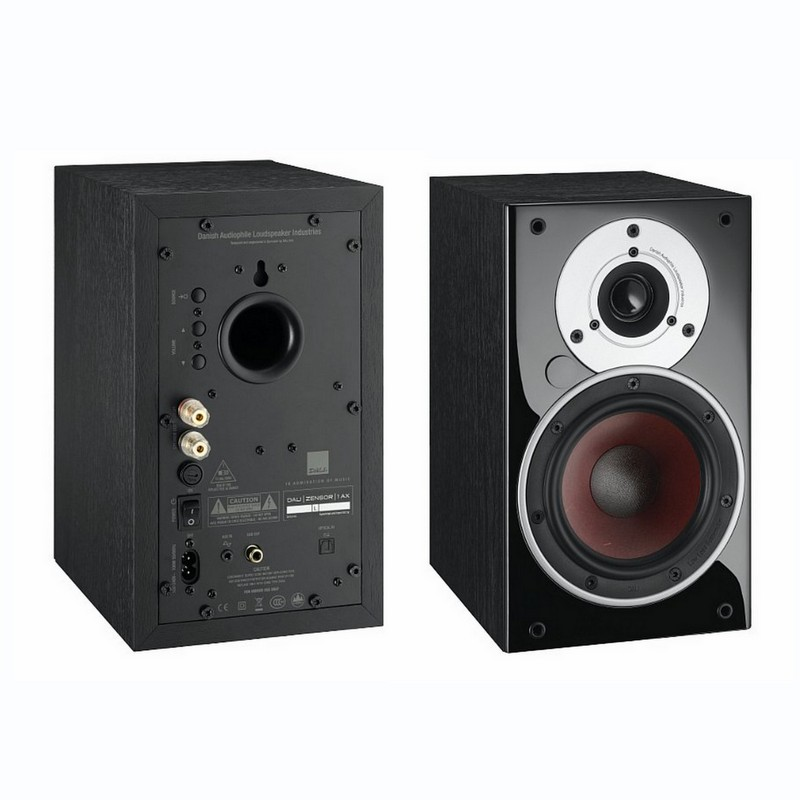
\includegraphics[width=0.6\textwidth]{figures/dali_zensor_1_ax.jpg}
\caption{The system will be developed upon the DALI Zensor 1 AX.}
\label{fig:dali_zensor}
\end{figure}

The specifications of the DALI Zensor 1 AX is as follows:

\begin{table}[H]
\centering
\begin{tabular}{ll}
\hline
Frequency Range (+/-3 dB) {[}Hz{]}            & 53 - 26.500                                                                  \\ \hline
Maximum SPL {[}dB{]}                          & 104                                                                          \\ \hline
Crossover Frequency {[}Hz{]}                  & 2.900                                                                        \\ \hline
Amplifier Type                                & Fully digital class D (Open loop type)                                       \\ \hline
Input Impedance {[}ohms{]}                    & 12.6k                                                                        \\ \hline
Connection Input                              & \begin{tabular}[c]{@{}l@{}}3.5mm mini jack \\ Optical (Toslink)\end{tabular} \\ \hline
Connection Output                             & SUB Out                                                                      \\ \hline
Max. Power Consumption {[}W{]}                & \begin{tabular}[c]{@{}l@{}}160W\\ \textless0.5W\end{tabular}                 \\ \hline
Dimensions With Base (HxWxD) {[}mm{]}         & 274 x 162 x 240                                                              \\ \hline
Weight {[}kg{]}                               & 4.6                                                                          \\ \hline
Analogue Input Sensitivity {[}mV{]}           & 300                                                                          \\ \hline
Continous IEC Amplifier Output {[}RMS watt{]} & 2 x 50                                                                       \\ \hline
Max. Digital Resolution {[}bits/KHz{]}        & 24 / 96                                                                      \\ \hline
\end{tabular}
\caption{DALI Zensor 1 AX specifications \citep{DaliSpec}}
\label{fig:dali_zensor_spec}
\end{table}

The DALI Zensor 1 AX will be the speaker used in this project given by DALI for the purpose of testbench and the speaker which the final system will be implemented in.